%% Notes for CETW 2025
%% DID with multiple periods

\documentclass[../didNotes.tex]{subfiles}

\begin{document}

\section{多期DID}

这部分笔记讨论多个时期情况下DID方法的识别、估计与推断。首先,我们考虑只有一个处理时点的情况,也就是所谓的简单事件研究法,
此时的DID设计中,ATT的识别无非是两期DID简单扩展到多个时期,这部分重点讨论的内容是如何理解平行趋势假设并对这一假设进行敏感性分析;
其次,我们考虑纳入协变量,这部分无非是两期DID纳入协变量的简单扩展。

然后,我们考虑多个处理发生在不同时点的情形(但是每个个体最多受到一次处理),也就是所谓的交错DID,这部分的关键在于,如何基于不同假设选择合适的控制组,
从而识别每个``处理--时点''所对应的ATT,并将其加总得到聚合的单一/截面/动态序列处理效应;接着,我们讨论交错DID设计下TWFE估计方法的问题;最后,
我们在交错DID情形下纳入协变量,这部分无非是多期DID纳入协变量的简单拓展。

\subsection{简单事件研究法}

假设有时期 $1,2, \ldots ,T$,唯一的处理发生在 $t=g$ 时期,个体的接受处理标志为 $D_{i} \in \{ g,\infty \}$,个体的潜在结果是
$$
Y_{i,t} = \mathbb{1} (D_{i}=g) Y_{i,t}(g) + \mathbb{1} (D_{i}=\infty)Y_{i,t}(\infty)
$$
这里我们用 $\infty$ 表示个体从未接受处理。``事件研究法''这个词的含义是,估计处理在发生后的每一期对于受到处理的个体的因果效应,这一因果效应
是相对于某个基期而言的(一般选择处理发生前一期为基期)也就是说,对于 $t: g \le t \le T$,我们希望来计算如下的每一期的平均处理效应所构成的序列:
$$
\text{ATT}(t) \coloneqq \mathbb{E}_{\omega}[Y_{i,t}(g) - Y_{i,t}(\infty) \mid D_{i}=g]
$$
从而我们有 $T-g+1$ 个未知参数需要做识别、估计和推断。

首先来考虑识别和估计问题,与两期DID一样,我们使用平行趋势假设(PT)来进行识别,但由于有多个参数需要识别,就需要多个平行趋势假设,如下
\begin{assumption}[PT-ES]\label{thm:pt-es}
  潜在结果 $Y_{i,g-1}(\infty)$ 到 $Y_{i,t}(\infty)$ 在处理组和控制组里的变化趋势对于 $t:g\le t\le T$ 在平均意义上是一样的,也就
  $$
  \mathbb{E}_{\omega}[Y_{i,t}(\infty) -Y_{i,g-1}(\infty) \mid D_i=g] =
  \mathbb{E}_{\omega}[Y_{i,t}(\infty) - Y_{i,g-1}(\infty) \mid D_i=\infty], \; \forall g \le t \le T
  $$
\end{assumption}
\autoref{thm:pt-es} 允许我们来识别整个平均处理效应序列,如果该假设只对于某些期 $t$ 成立,那么我们可以识别出这些期的平均处理效应,也就是
\begin{align*}
  \text{ATT}(t) &= \mathbb{E}_{\omega}[Y_{i,t}(g)-Y_{i,g-1}(\infty) \mid D_{i}=g] -
  \mathbb{E}_{\omega}[Y_{i,t}(\infty)-Y_{i,g-1}(\infty) \mid D_{i}=\infty] \\
  &= \mathbb{E}_{\omega}[Y_{i,t}-Y_{i,g-1} \mid D_{i}=g] -
  \mathbb{E}_{\omega}[Y_{i,t}-Y_{i,g-1} \mid D_{i}=\infty]
\end{align*}
从而这一识别所对应的估计量可以很容易地写出来
$$
\widehat{\text{ATT}}(t) = (\bar{Y}_{\omega, D=g, t}-\bar{Y}_{\omega, D=g, g-1}) -
(\bar{Y}_{\omega, D=\infty, t}-\bar{Y}_{\omega, D=\infty, g-1})
$$
也就是用样本加权平均值代替条件期望。在估计出动态平均处理效应序列后,可以对时间序列取平均,得到一个对时间而言``平均''的平均处理效应
$$
\widehat{\text{ATT}} \equiv \frac{1}{T-g+1} \sum_{t=g}^{T} \widehat{\text{ATT}}(t)
$$
从而一目了然地看出处理的平均效果。

其次,我们来做推断。文献中建议的方法是将上述估计结果写成等价的TWFE形式
$$
Y_{i,t} = \alpha_i + \eta_t + \sum_{k=1}^{g-2} \beta_k \left[ \mathbf{1}(G_i=g)
\mathbf{1}(t=k) \right] +
\sum_{s=g}^{T} \beta_s  \left[ \mathbf{1}(G_i=g) \mathbf{1}(t=s) \right] + \epsilon_{i,t}
$$
可以简单地证明,$\beta_{k}=\tau_{k},\beta_{s}=\text{ATT}_s$。因此,可以利用我们所熟悉的线性回归的大样本性质来构建渐进统计量,对平均
处理效应进行假设检验。基于bootstrap的检验方法可以用\texttt{csdid}软件包实现。%% TODO 写证明过程,以及静态TWFE-DID估计量的含义

\subsection{平行趋势检验}

接下来,我们来更加仔细地审视对于DID识别至关重要的平行趋势假设。目前的实证文章中,通常会通过对处理发生前趋势差异做假设检验,来``检验''平行趋势假设。
事前趋势差异 $\tau_{-k}$ 定义为
\begin{align*}
  \tau_{-k} &\coloneqq \mathbb{E}[Y_{i,t=g-1-k}(\infty)-Y_{i,t=g-1}(\infty) \mid D_i = g] -
  \mathbb{E}[Y_{i,t=g-1-k}(\infty)-Y_{i,t=g-1}(\infty) \mid D_i = \infty] \\
  &= \mathbb{E}[Y_{i,t=g-1-k}-Y_{i,t=g-1} \mid D_i = g] -
  \mathbb{E}[Y_{i,t=g-1-k}-Y_{i,t=g-1} \mid D_i = \infty], 0 < k < g-1
\end{align*}
其含义是处理发生前的第 $k$ 期的结果变量到 $g-1$ 期在处理组和控制组里的平均变化趋势之差,若为0,则说明 $k \to g-1$ 期两组的趋势无差异,若
全部为0,则说明处理发生前,处理组和控制组的结果变量的平均演化过程。因此,对 $\tau_{-k}$ 的估计量做假设检验,
若无法拒绝每一期的事前趋势差异为0的原假设,则认为平行趋势假设成立?

上述陈述是有争议的。这一检验最大的问题是:平行趋势是对观测不到的潜在因果的演化趋势做出的假设,因此本身是不可检验的。上述检验只能为平行趋势假设的
成立与否提供一些信息,但是,最近的文献指出,由于多重假设检验、检验效力和处理的选择机制等问题,这一检验所包含的信息会含有噪声,妨碍我们对于结果的理解。
处于稳健性的考量,文献也建议实证研究者在汇报结果时,对可能违反PT的情况做一些敏感性分析,增加结果的可信度。

\textbf{争议一,处理的选择机制导致事前检验失效}。\textcite{ghanem2025} 研究了这一问题。这里我们仅仅讨论原文中涉及的一种情况(处理选择机制),
也就是个体会根据当期实现的未观测冲击来决定是否接受处理(所谓的不完美前瞻,imperfect foresight),而不关心未来的不确定性冲击。
为了进行一些理论分析,文章假设了处理的选择机制 $D_{i}$ 为不可观测随机变量的函数
$$
D_{i} = g(\alpha_{i},\epsilon_{i 1}, \epsilon_{i 2}, \nu_{i}, \eta_{i 1}, \eta_{i 2})
$$
其中,$\alpha, \epsilon$ 可以理解为固定效应和随机扰动项,他们也决定了潜在结果
$$
Y_{i t}(0) = \xi_{t}(\alpha_{i}, \epsilon_{i t})
$$
而 $\nu,\eta$ 是一组额外的未观测随机变量。这些变量的实现值分别用 $a,e,v,t$ 来表示。不完美前瞻的处理选择机制指的是如下函数类
$$
\mathcal{G}_{\text{if}} \coloneqq \{ g: \exists g', g(\alpha_{i},\epsilon_{i 1}, \epsilon_{i 2}, \nu_{i},
\eta_{i 1}, \eta_{i 2}) = g'(\alpha_{i},\epsilon_{i 1}, \nu_{i}, \eta_{i 1}) \}
$$
当上述选择机制存在时,平行趋势假设满足需要一些额外条件。\textcite{ghanem2025} 所展示的一个必要条件是:
$$
\text{PT} \implies \mathbb{E}[Y_{i 2}(0)-\mathbb{E}[Y_{i 2}(0)] \mid \alpha_{i},\epsilon_{i 1}] = Y_{i
1}(0)-\mathbb{E}[Y_{i 1}(0)] \; \textit{a.s.}
$$
如果把 $Y_{i t}(0) - \mathbb{E}[Y_{i t}(0)]$ 看作一个关于 $t$ 的随机过程,那么这个随机过程具有鞅性质:下一期的期望等于当期的实现值。

可以进一步将上述条件写成
$$
Y_{i 2}(0) - Y_{i 1}(0) = \mathbb{E}[Y_{i 2}(0) - Y_{i 1}(0)] + \zeta_{i t}, \; \mathbb{E}[\zeta_{i t} \mid
\alpha_{i},\epsilon_{i t}]=0
$$
That is, Proposition 3.2 allows the each individual's untreated potential outcomes to vary over time beyond
deterministic mean shifts but requires the stochastic component of the change over time, $\zeta_{i 2}$,
to be mean-independent of the pre-treatment unobservables $(\alpha_{1},\epsilon_{i 1})$

进一步,可以证明存在上述选择机制时(以及线性放松的鞅条件下),用平行趋势假设识别出来的ATT会具有误差
\begin{align*}
  \Delta_{\text{post}} &= \Delta_{\text{post}}^{\text{sel}} + \Delta_{\text{post}}^{\text{mtg}} \\
  &= \mathbb{E}[\zeta_{i 2} \mid D_{i}=1] - \mathbb{E}[\zeta_{i 2} \mid D_{i}=0] \\
  &+ (\rho_{2}-1) \left(\mathbb{E}[Y_{i 1} \mid D_{i}=1] - \mathbb{E}[Y_{i 1} \mid D_{i}=0]\right)
\end{align*}
其中,$\rho_{2}$ 满足 $\mathbb{E}[\dot{Y}_{i 2}(0) \mid \alpha_{i}, \epsilon_{i 1}]=\rho_{2} \dot{Y}_{i 1}$.
可以看到,误差分为两部分,第一部分是两组之间第二期随机冲击项的均值之差,若处理与第二期的随机冲击的实现值相关,那么第一部分将不为0;第二部分
是鞅条件偏离程度 $\rho_{2}-1$ 和两组结果之间的事前差异,如果鞅条件偏离程度越远,那么即使我们检验出一个很小的事前差异,
也会给DID的识别带来很大的偏差。

另一种典型处理选择机制是基于固定效应的选择,考虑结果模型 $Y_{i t}(0) = \theta_{i} \gamma_{t}$
与处理选择模型 $D_{i} = \theta_{i}$,其中,$\gamma_{t}$ 是随着时间增长的趋势项,$\theta_{i} \in \{ 0,1 \}$ 是某种固定效应。
此种情况下,只要两组个体潜在结果的时间趋势项不一样,也就是 $\gamma_{2} \neq \gamma_{1}$,平行趋势将无法满足,因为
$$
\mathbb{E}[Y_{i 2}(0) - Y_{i 1}(0) \mid D_{i}=1] - \mathbb{E}[Y_{i 2}(0) - Y_{i 1}(0) \mid D_{i}=0] =
\gamma_{2} - \gamma_{1}
$$
将这一两期模型推广到多期,显然存在处理后平行趋势不满足的问题,在这种情况下,事前趋势检验能否将这一问题检验出来呢?更正式地提出这个问题:
给定一个存在趋势偏离的结果模型,如果事后趋势偏离足够大以至于使得平均处理效应不显著,其事前趋势是否能够被传统的检验方法检验出来?
我们在下面的第二个争议部分进行讨论。

\textbf{争议二,事前检验效力不足,无法为事后趋势提供有意义的参考}。\textcite{roth2022} 指出,常用的事前趋势检验方法存在检验效力低的问题,
即使确实存在事后非平行趋势,事前趋势检验也无法将其识别出来。Roth做了一个文献分析和数值模拟,它假设这些文献估计得到的处理效应系数符合如下数据生成过程
$$
\hat{\beta} \sim \mathcal{N}(\beta, \Sigma)
$$
其中,$\beta$ 是真实处理效应 $\tau$ 加上一个趋势偏差 $\delta$
$$
\beta =
\begin{pmatrix}
  \delta_{\text{pre}} \\
  \delta_{\text{post}}
\end{pmatrix} +
\begin{pmatrix}
  0 \\
  \tau_{\text{post}}
\end{pmatrix}
$$
这一分解表明,实际情形是:事前事后都有趋势差异,事前没有处理效应,事后有处理效应 $\tau_{\text{post}}$,并且无法被识别出来。Roth将估计量分布的
方差-协方差矩阵校准到文献中汇报的结果,希望研究的是:在上述确实存在事后趋势的DGP中,事前检验是否能把事后趋势检验出来?为了使研究更方便,作者假设
事前事后趋势的偏离均符合线性,也就是 $\delta_{t} = \gamma t$,并定义``检验通过''指的是事前系数估计值 $\hat{\beta}_{\text{pre}}$ 满足
$$
\hat{\beta}_{\text{pre}} \in B_{\text{NIS}}(\Sigma) = \{ \beta \in \mathbb{R}^{K}: \left\vert \beta_{t}
\right\vert  \le 1.96 \sigma_{t} \}
$$
显然,这个集合的含义是系数在5\%的水平上不显著为0,接受系数为0的原假设。现在。Roth选择了趋势偏离系数 $\gamma = \gamma_{0.8}$ 使得
$\Pr(\hat{\beta}_{\text{pre}} \notin B_{\text{NIS}} \mid \delta_{\text{post}} \neq 0) = 0.8$,
也就是说,使得事前趋势检验的效力(power)为0.8(在这个DGP中,检验出事前趋势等价于检验出事后趋势)。
在这一事前检验的设定下,我们来看事后参数估计的偏差以及检验的显著性水平(size),暂且考虑``条件于通过事前检验''的版本
\begin{align*}
  \text{bias} &\equiv \mathbb{E}[l' \hat{\beta}_{\text{post}} - l' \tau_{\text{post}} \mid
  \hat{\beta}_{\text{pre}} \in B_{\text{NIS}}] \\
  \text{size} &\equiv \mathbb{E}[l' \tau_{\text{post}} \notin \text{CI}_{\tau} \mid \hat{\beta}_{\text{pre}}
  \in B_{\text{NIS}}]
\end{align*}
其中,bias指的是事前趋势检验通过时,DID估计量的偏差;size指的是事前趋势检验通过时,即使真实的处理效应为0,仍然认为处理效应不为0的概率
(实际上就是拒绝了事后估计系数为0的原假设,犯了第一类错误)。

现在,我们再来总结一下Roth到底在干什么。他的核心目标是:说明在存在事后趋势的情况下,事前趋势检验也会很容易通过,从而无法为PT的违反提供足够的信息,
造成DID估计量的偏差。为了说明这一点,作者假设了一个线性违反PT的DGP(容易看出,就是第一个争议中所说的基于非观测固定效应的选择),
并手动设定其偏离系数,使得在80\%的情况下能够检验出事前趋势,从而观察在这一情况下,DID估计量的偏差和显著性检验时犯第一类错误的概率。
结果见 \autoref{pic:PT_bias}

\begin{figure}[htbp]
  \begin{center}
    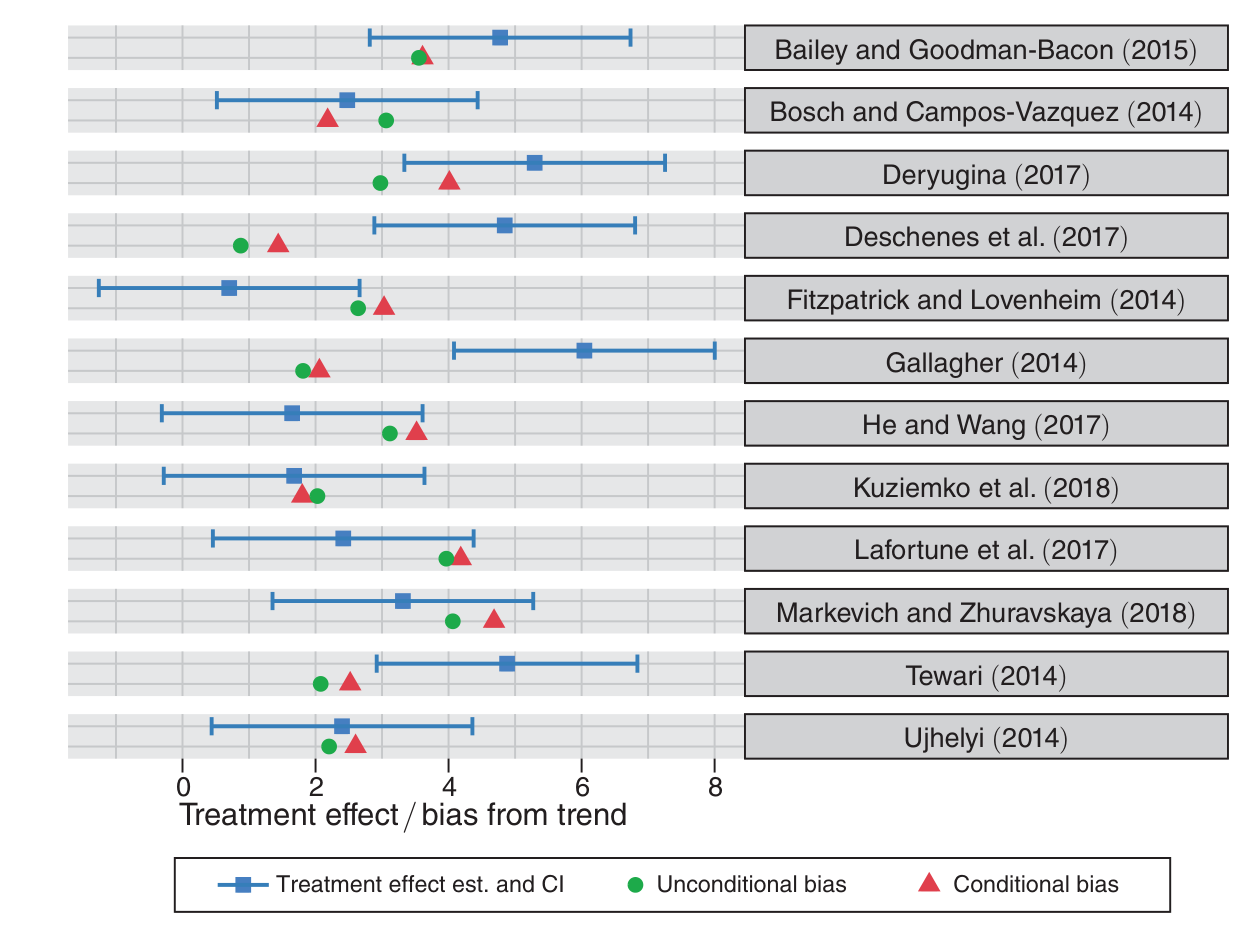
\includegraphics[width=0.75\textwidth]{./assets/PT_caution.png}
  \end{center}
  \caption{PT违反情形下DID估计量的偏差}
  \label{pic:PT_bias}
\end{figure}

可以看到结果令人震惊:当PT的违反足够大,以至于能够使得事前趋势检验在80\%的情况下检验出非平行趋势的时候,许多DID估计量的偏差甚至在绝对值上
超过了估计量本身!这还是在PT违反比较大的情况下,可想而知,如果PT的违反稍微小一点,那么事前趋势的检验效力将进一步降低,而DID估计量的偏差仍然会
足以影响估计的显著性。上述数值模拟提供了一个反例:许多情况下,平行趋势的违反没有大到足以被我们检验出来,却仍然会影响估计量的显著性。这一问题发生的
主要原因是:
\begin{itemize}
  \item 事前趋势检验是做多个t检验,单独做t检验效力低,无法检验出那种单期来看不显著,但是多期累积起来就会形成趋势的情况
  \item 聚类计算标准误时,标准误会变大,使得事前检验不容易显著
  \item 小样本下存在多重假设检验问题
\end{itemize}

由于这些问题的存在,\textcite{rambachan2023} 提出了一种对PT可能的违反做敏感性分析的方法,以及相应的软件包 \texttt{HonestDID}。
这个方法采用了先验假设+部分识别技术,就是在看存在特定的PT违反时,事后估计系数和显著性会怎么变化,同时报告这一结果。当然,由于没有什么理论来支撑,
我们不知道给什么样的假设是合适的,所以这一方法并没有完全解决平行趋势检验的问题。

\textcite{rambachan2023} 的主要想法是,将PT假设放松到``PT被违反,但是违反程度在一定范围内'',也就是将趋势偏离 $\delta$ 限制在某个集合
$\Delta$ 中,这个集合需要根据先验知识去选取,他们提出的一种比较通用的集合是``凸多面体约束''(在线性规划中常用)
$$
\delta \in \Delta \equiv \{ \delta: A \delta \le d \}
$$
其中 $A,d$ 是事先选取的超参数矩阵和向量。这一约束包含了许多常用情况,例如relative magnitudes
$$
\Delta^{\text{RM}}(M) = \{ \delta: \forall t \ge 0,\left\vert \delta_{t+1}-\delta_{t} \right\vert \le M \cdot
\max_{s<0} \left\vert \delta_{s+1}-\delta_{s} \right\vert  \}
$$
在这个约束中,事后趋势偏离不会超过事前趋势偏离最大值的 $M$ 倍。\textcite{rambachan2023} 的理论贡献是推导了在类似平行趋势被
有限度地违反地情况下,如何构造置信区间并进行推断,他们用这一方法对文献进行了敏感性分析,如 \autoref{pic:PT_sensitivity} 所示
\begin{figure}[htbp]
  \begin{center}
    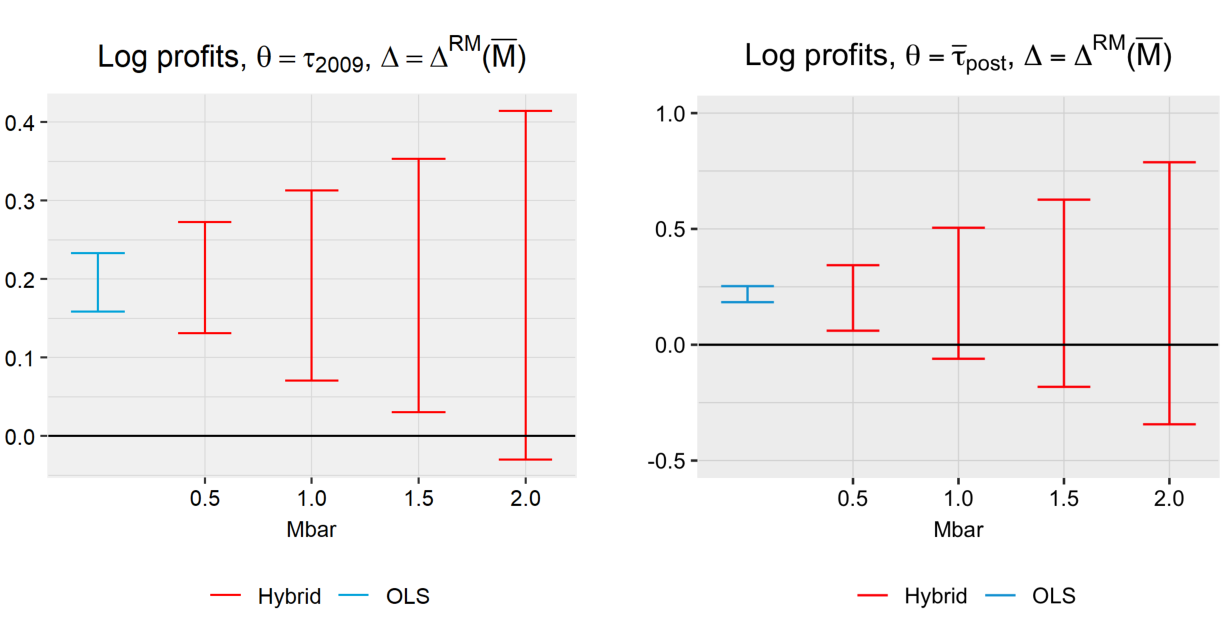
\includegraphics[width=0.85\textwidth]{./assets/PT_sensitivity.png}
  \end{center}
  \caption{对Benzarti and Carloni (2019) 的敏感性分析}
  \label{pic:PT_sensitivity}
\end{figure}
可以看到,问题在于我们不知道什么样的 $M$ 的选取是有意义的,缺乏一个比较的框架。

\subsection{加入协变量}

在简单事件研究法中加入协变量,无非是吧两期情况下的条件PT假设扩展到多期(相对于基期),然后根据多期相对于基期构造多个RA、IPW和DR估计量,然后计算
方差,进行推断。这里的问题是,不能用TWFE做估计和推断了,因为TWFE对于CATT的加总使用的权重是不清楚的。这部分相对于两期DID而言没有任何新内容,
因此简单略过。除了一点,在带有协变量的情况下,如何检查平行趋势呢?

%% TODO inference and PT with covariates

\subsection{交错DID}

我们需要进一步修改潜在因果框架的形式以适应交错处理的情况。直觉上,``交错处理''实际上就是许多不同的\( 2 \times 2 \) 处理-对照比较。
假设每个个体最多只会接受一次处理,且处理不会被取消。我们用处理开始的日期来索引潜在结果,记为 \( g: Y_{i,t}(g) \);对于永不接受处理的个体,
我们用 \( Y_{i,t}=Y_{i,t}(\infty) \) 来表示。因此,潜在结果可以表示为
\[
  Y_{i,t} = \sum_{g \in \mathcal{G}} Y_{i,t}(g) \mathbf{1}(G_{i}=g)
.\]
其中 \( \mathcal{G} \) 表示所有处理时间的集合。举例来说,假设有四期、两个处理和三个个体的数据,
且处理分别发生在第二期和第三期,那么数据结构为
\begin{align*}
  Y_{1,1}(\infty),Y_{1,2}(\infty),Y_{1,3}(\infty),Y_{1,4}(\infty) \\
  Y_{2,1}(2), Y_{2,2}(2), Y_{2,3}(2), Y_{2,4}(2) \\
  Y_{3,1}(3), Y_{3,2}(3), Y_{3,3}(3), Y_{3,4}(3)
\end{align*}

与之前一样,我们需要一个“无预期”的假设,以精确定义处理日期并维持 PT 假设:
对于所有最终被处理的个体 \( i \),以及所有特定的处理前时期 \( t < g \) 而言,有
\[
  Y_{i,t}(g) = Y_{i,t}(\infty)
.\]

\textbf{识别并估计group-time ATT}。现在我们讨论在交错情形下,\( t \) 时刻的ATT识别与估计。在交错 DID 设计中,
每一个处理组(或处理队列,由处理时间定义)都有自己的处理效应参数序列。我们称之为组-时间平均处理效应(group-time ATT)
\[
  \text{ATT}(g,t) \coloneqq \mathbb{E}_{\omega}[Y_{i,t}(g)-Y_{i,t}(\infty) \mid G_i = g]
.\]
在这一表示中要求 \( t \ge g \)。若 \( t < g \),则是一个处理前参数,可以用于检验PT。
需要注意的是,\( Y_{i,t}(\infty) \mid G_i=g \) 是反事实结果,因而无法从数据中直接得到。这正是PT假设发挥作用的地方。

在交错 DID 设计中,我们需要选择哪些个体作为对照组。一般有两种选择:从未接受处理的个体(never-treated),
以及尚未接受处理的个体(not-yet-treated)。我们所做的 PT 假设将取决于所选择的对照组
\begin{assumption}[基于从未接受处理个体的 PT,NEV]\label{thm:pt-nev}
  对于所有最终会接受处理的组 \( g \) 和处理后时期 \( t \ge g \),有
  \[
    \mathbb{E}_{\omega}[Y_{i,t}(\infty)-Y_{i,t-1}(\infty) \mid G_i=g] =
    \mathbb{E}_{\omega}[Y_{i,t}(\infty)-Y_{i,t-1}(\infty) \mid G_i=\infty]
  .\]
\end{assumption}

\begin{assumption}[基于尚未接受处理个体的 PT,NYT]\label{thm:pt-not-yet}
  对于所有最终会接受处理的组 \( g \),尚未接受处理的组 \( g' \),以及处理后时期
  \( t: g \le t < g' \),有
  \[
    \mathbb{E}_{\omega}[Y_{i,t}(\infty)-Y_{i,t-1}(\infty) \mid G_i=g] =
    \mathbb{E}_{\omega}[Y_{i,t}(\infty)-Y_{i,t-1}(\infty) \mid G_i=g']
  .\]
\end{assumption}

一些文献还使用更严格的PT假设——要求PT在所有时期和所有组中都成立——以构造更精确的估计量
\begin{assumption}[所有时期与所有组的 PT,ALL]\label{thm:pt-all}
  对于任意两个组 \( g,g' \) 和时期 \( t \),有
  \[
    \mathbb{E}_{\omega}[Y_{i,t}(\infty)-Y_{i,t-1}(\infty) \mid G_i=g] =
    \mathbb{E}_{\omega}[Y_{i,t}(\infty)-Y_{i,t-1}(\infty) \mid G_i=g']
  .\]
\end{assumption}

利用 \autoref{thm:pt-nev},我们可以很快得到
\[
  \mathbb{E}_{\omega}[Y_{i,t}(\infty)-Y_{i,g-1}(\infty) \mid G_i=g] =
  \mathbb{E}_{\omega}[Y_{i,t}(\infty)-Y_{i,g-1}(\infty) \mid G_i=\infty]
.\]
将其代入 \( \text{ATT}(g,t) \) 得到
\[
  \text{ATT}(g,t) = \mathbb{E}_{\omega}[Y_{i,t}-Y_{i,g-1} \mid G_i=g] -
  \mathbb{E}_{\omega}[Y_{i,t}-Y_{i,g-1} \mid G_i=\infty]
.\]
由此可以识别。结合前面的例子,这个估计量可以构造为
\begin{align*}
  \widehat{\text{ATT}}(2,2)&=[Y_{2,2}-Y_{2,1}] - [Y_{1,2}-Y_{1,1}] \\
  \widehat{\text{ATT}}(3,3)&=[Y_{3,3}-Y_{3,1}] - [Y_{1,3}-Y_{1,1}]
  .
\end{align*}
等等。采用NEV假设时,也可以使用如下fully saturated回归来估计ATT,估计结果与手动计算的DID估计量是一样的
$$
Y_{i,t} = \alpha_{i} + \eta_{t} + \sum_{g \neq \infty} \sum_{e \neq -1} \beta_{g,e} \mathbb{1} (G_{i}=g)
\mathbb{1}(G_{i}+e=t) + \epsilon_{i,t}
$$

利用 \autoref{thm:pt-not-yet} 可以识别 ATT:
\[
  \text{ATT}(g,t) = \mathbb{E}_{\omega}[Y_{i,t}-Y_{i,g-1} \mid G_i=g] -
  \mathbb{E}_{\omega}[Y_{i,t}-Y_{i,g-1} \mid G_i > \max \{g,t\} ]
.\]
结合前面的例子,该估计量可以构造为
\begin{align*}
  \widehat{\text{ATT}}(2,2) &= [Y_{2,2}-Y_{2,1}] - \frac{1}{2} [Y_{1,2}-Y_{1,1} +
  Y_{3,2}-Y_{3,1}] \\
  .
\end{align*}
其他情况与NEV估计量相同。

基于 \autoref{thm:pt-all} 的估计量暂时略去。交错情况下的估计方法与简单事件研究法完全一致,只不过需要明确对哪一个队列和时间点去估计,
以及明确使用谁作为控制组。因此估计的具体表达式也略去了,只是用上面的例子来说明。
估计的具体表达式和推断方法(计算标准误)可以参考 \textcite{callaway2021}。

%% TODO try to add the PT-ALL case, focus on Wooldridge's papers

\textbf{将group-time ATT进行加总}。在识别并估计出group-time ATT后,我们发现这些结果太多了,希望得到一些加总的结果,来系统地描述这个处理
所产生的总体情况或者平均影响。直觉上,有三种加总方式:一是对所有时间和组进行加总,代表处理发生后的整体影响;
二是在某个时间截面上对所有组的情况进行加总,得到处理发生特定时间后,对所有组的平均影响;
三是对某个组的处理效应时间序列进行加总,得到该处理对于某个组(相对于其对照组而言)的平均影响。我把三类加总方式列在下面:
\begin{itemize}
  \item 所有处理个体与时间的平均效应:\( \text{ATT}_{\text{agg}}
    \coloneqq \sum_{g,t} w_{\omega, g,t} \text{ATT}(g,t) \)
  \item 事件发生后 \( e \) 期的平均效应:\(
      \text{ATT}_{\text{es}}(e) \coloneqq \sum_{g < \infty} w^{\text{es}}_{\omega, g, e}
    \text{ATT}(g,g+e)  \)
  \item 特定队列的平均效应:\( \text{ATT}_{\text{es}}(g) \coloneqq
    \sum_{0 \le e \le T-g} w^{\text{es}}_{\omega, g, e} \text{ATT}(g,g+e)  \)
\end{itemize}

\textbf{交错情形下加入协变量}。无非是把上面的difference-in-mean交错DID估计改成RA、IPW和DR三个版本,这里也略去了。估计量的性质还是参见
\textcite{SantAnna.Zhao2020, callaway2021}

\subsection{TWFE的问题}

许多情形下,使用TWFE来估计DID设计所对应的ATT不是一个好的选择。下面,我们来对这个问题进行分类讨论

\begin{table}[ht]
  \caption{TWFE可用性比较}\label{tab:TWFE}
  \centering
  \begin{adjustbox}{width = \textwidth, center}
    \begin{tabular}{@{} l*{3}{c} @{}}
      \toprule
      DID设计    & 简单回归       & 灵活回归   & 文献    \\
      \hline
      两期    & $\checkmark$     & --   & --  \\
      两期带协变量    & $\times$     & --  & \textcite{SantAnna.Zhao2020}   \\
      多期    & $\checkmark$ (minus pre-effect)     & $\checkmark$ & --    \\
      多期带协变量    & $\times$     & $\times$  & \textcite{callaway2021}   \\
      交错-NEV    & $\times$   & $\checkmark$ (IW) & \textcite{sun2021}    \\
      交错-NYT    & $\times$    & $\checkmark$ (IW, last-treated) & \textcite{sun2021}    \\
      交错-ALL    & $\times$    & $\checkmark$ (ETWFE) & \textcite{wooldridge2021}   \\
      交错带协变量    & $\times$    & $\times$ & \textcite{callaway2021} \\
      \bottomrule
    \end{tabular}
  \end{adjustbox}
\end{table}

\end{document}
